\documentclass[tikz,border=8pt]{standalone}
\usepackage{amsmath}
\usetikzlibrary{arrows.meta,decorations.pathmorphing,patterns}
\begin{document}
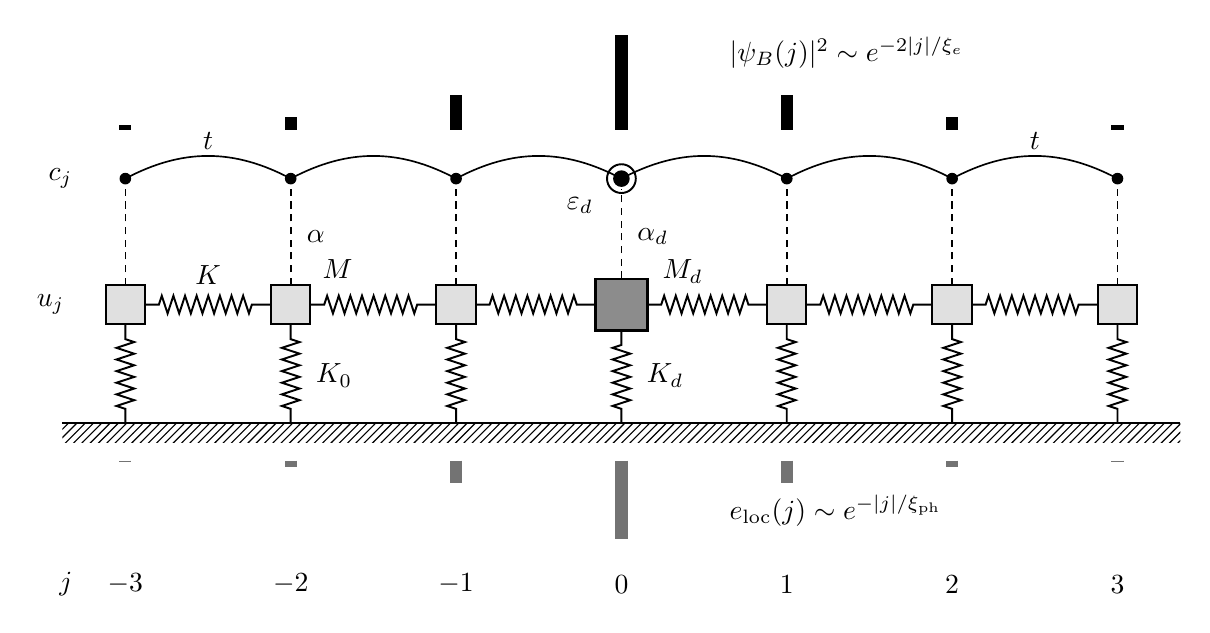
\begin{tikzpicture}[
  spring/.style={line width=.7pt,decorate,
    decoration={zigzag,segment length=4.2pt,amplitude=3.2pt,pre length=5pt,post length=5pt}},
  bar/.style={line width=4.4pt},
  hop/.style={line width=.6pt},
  coupling/.style={line width=.6pt,dash pattern=on 2.6pt off 2pt}]
  \def\dx{2.1}
  % Fixed ground for the on-site springs K_0 (K_d at the defect).
  \fill[pattern=north east lines] (-7.1,0.25) rectangle (7.1,0.5);
  \draw[line width=.8pt] (-7.1,0.5) -- (7.1,0.5);
  % On-site springs, electron-lattice coupling lines and electron sites.
  \foreach \j in {-3,...,3} {
    \pgfmathsetmacro{\x}{\j*\dx}
    \pgfmathsetmacro{\h}{ifthenelse(\j==0,0.33,0.25)}
    \draw[spring] (\x,0.5) -- (\x,2-\h);
    \draw[coupling] (\x,2+\h) -- (\x,3.47);
    \node at (\x,-1.55) {$\j$};
  }
  % Nearest-neighbour springs K between the oscillators.
  \foreach \j in {-3,...,2} {
    \pgfmathsetmacro{\xa}{\j*\dx+ifthenelse(\j==0,0.33,0.25)}
    \pgfmathsetmacro{\xb}{(\j+1)*\dx-ifthenelse(\j==-1,0.33,0.25)}
    \draw[spring] (\xa,2) -- (\xb,2);
    \draw[hop] (\j*\dx,3.6) to[bend left=28] ({(\j+1)*\dx},3.6);
  }
  % Host oscillators (mass M) and the defect oscillator (mass M_d).
  \foreach \j in {-3,-2,-1,1,2,3} {
    \filldraw[fill=black!12,line width=.7pt] ({\j*\dx-0.25},1.75) rectangle ({\j*\dx+0.25},2.25);
  }
  \filldraw[fill=black!45,line width=.8pt] (-0.33,1.67) rectangle (0.33,2.33);
  % Electron sites; the defect site carries the potential epsilon_d.
  \foreach \j in {-3,-2,-1,1,2,3} { \fill (\j*\dx,3.6) circle (2.1pt); }
  \fill (0,3.6) circle (3pt);
  \draw[line width=.7pt] (0,3.6) circle (5.2pt);
  % Bound-state density above the chain, local vibrational mode below it.
  \foreach \j/\p/\e in {-3/0.06/0.02,-2/0.16/0.08,-1/0.44/0.29,0/1.20/1.00,1/0.44/0.29,2/0.16/0.08,3/0.06/0.02} {
    \draw[bar] (\j*\dx,4.22) -- (\j*\dx,4.22+\p);
    \draw[bar,black!55] (\j*\dx,0.02) -- (\j*\dx,0.02-\e);
  }
  % Labels (mathematical notation only).
  \node[anchor=west] at (1.25,5.2) {$|\psi_B(j)|^2\sim e^{-2|j|/\xi_e}$};
  \node[anchor=west] at (1.25,-0.62) {$e_{\mathrm{loc}}(j)\sim e^{-|j|/\xi_{\mathrm{ph}}}$};
  \node at (-5.25,4.08) {$t$};
  \node at (5.25,4.08) {$t$};
  \node[anchor=east] at (-0.24,3.26) {$\varepsilon_d$};
  \node[anchor=west] at (0.08,2.86) {$\alpha_d$};
  \node[anchor=west] at (-4.12,2.86) {$\alpha$};
  \node[anchor=west] at (0.4,2.42) {$M_d$};
  \node[anchor=west] at (-3.92,2.45) {$M$};
  \node at (-5.25,2.38) {$K$};
  \node[anchor=west] at (0.2,1.1) {$K_d$};
  \node[anchor=west] at (-4.0,1.1) {$K_0$};
  \node[anchor=east] at (-6.85,3.6) {$c_j$};
  \node[anchor=east] at (-6.95,2.0) {$u_j$};
  \node[anchor=east] at (-6.85,-1.55) {$j$};
\end{tikzpicture}
\end{document}
